% PRISM-3D manuscript. Compile: pdflatex main && bibtex main && pdflatex main && pdflatex main
% Every value that comes from an experiment is written as \xyz (yellow) until the pipeline is run.
% Fill them with scripts/fill_results.py (see docs/filling_results.md).
% For submission to an Elsevier journal, move the body into the elsarticle template unchanged.
\documentclass[11pt,a4paper]{article}
\usepackage[utf8]{inputenc}
\usepackage{mathptmx} % Times; on Overleaf you may use \usepackage[T1]{fontenc}\usepackage{lmodern} instead
\usepackage[margin=2.4cm]{geometry}
\usepackage{amsmath,amssymb}
\usepackage{graphicx}
\usepackage{booktabs}
\usepackage{tabularx}
\usepackage{multirow}
\usepackage{xcolor}
\usepackage[round,authoryear]{natbib}
\usepackage{caption}
\usepackage{subcaption}
\usepackage[hidelinks]{hyperref}
\usepackage{setspace}
\setstretch{1.12}
\graphicspath{{figures/}}

% Result placeholder: replace every \xyz with the value from the result files.
% Each placeholder carries a key, e.g. \xyz[h1.bfree.delta]. The key names the value; it is not printed.
% python scripts/fill_results.py fills every key it can compute and lists all keys in paper_values.md.
\newcommand{\xyz}[1][]{\colorbox{yellow}{[xyz]}}
\newcommand{\feat}[1]{\texttt{#1}}

\title{Does Explicit Monocular 3D Geometry Help AI Generated Image Detectors?\\ A Controlled Study on Unseen Generators}
\author{[Author names]\thanks{[Affiliations and corresponding author email]}}
\date{}

\begin{document}
\maketitle

\begin{abstract}
Detectors of AI generated images often score well on familiar benchmarks and then lose much of their accuracy on images from new generators or images that have been compressed and resized on their way through the web. Physical cues offer a possible remedy: a photograph is a projection of a real scene, so its shading, perspective and occlusions should agree with one underlying 3D geometry, while a generator only imitates these regularities in two dimensions. Earlier work showed such violations by hand or with line and shadow annotations, but it remains unknown whether they add anything to current detectors. We test this question directly. We compute 26 explicit geometry features from frozen monocular estimators (MoGe, Depth Anything V2, DSINE and an ordinal shading decomposition), grouped into four cues: agreement between depth and surface normals, consistency of shading with the estimated shape, perspective consistency, and alignment of depth and image edges. We add them to three released detectors (B-Free, CO-SPY and UnivFD) through a calibrated logistic stacker fitted only on a separate pool of generators, and evaluate on four test sets whose generators and real image sources never appear in fitting: open models (FLUX, SD3, PixArt, Playground), a content matched set built from RAISE captions, the newest commercial systems in OpenFake, and an in the wild set. A DINOv2 control separates geometric signal from the effect of adding a strong visual backbone, and generator level cluster bootstrap intervals quantify uncertainty about new generators. Adding geometry changed macro AUROC on unseen generators by \xyz[h1.bfree.delta]{} (95\% CI \xyz[h1.bfree.ci]) for B-Free, \xyz[h1.cospy.delta]{} for CO-SPY and \xyz[h1.univfd.delta]{} for UnivFD. The gain \xyz[h2.abstract_verb]{} the DINOv2 control, \xyz[h3.abstract_verb]{} on content matched images and \xyz[h4.abstract_verb]{} under JPEG compression and resizing. We release the code, splits and feature tables.
\end{abstract}

\noindent\textbf{Keywords:} AI generated image detection; synthetic image forensics; monocular geometry; physical consistency; generalization; calibration; cluster bootstrap

% =====================================================================
\section{Introduction}
\label{sec:intro}

Text to image generators now produce photographs that people cannot reliably tell apart from real ones. In a large human study, participants misclassified 38.7\% of AI generated images \citep{lu2023seeing}. Automatic detectors are the practical answer, and their reported accuracy is often impressive. The difficulty is that this accuracy rarely survives contact with new generators. A detector trained on one family of models learns traces that are specific to that family, and when the test images come from a newer generator or have been compressed by a social network, performance drops sharply \citep{corvi2023detection,ojha2023univfd}. Recent benchmarks built from realistic images make the gap visible: detectors with high laboratory scores fall close to chance on the Chameleon set \citep{yan2025aide}, and the eleven detectors evaluated in AIGIBench lose much of their accuracy on images from social media and AI art platforms \citep{li2025aigibench}.

Most detectors rely on one of three kinds of evidence. Low level detectors look for traces of upsampling and spectral artifacts \citep{wang2020cnnspot,frank2020frequency,tan2024npr}. Foundation model detectors use features from large pretrained encoders such as CLIP \citep{ojha2023univfd,koutlis2024rine,yan2025effort}. Reconstruction detectors measure how well an image is reproduced by a generator's own autoencoder \citep{wang2023dire,ricker2024aeroblade}. Each kind fails in a known way: low level traces disappear under compression, semantic features miss subtle high fidelity images, and reconstruction errors are tied to one generator family. Hybrid detectors that combine semantic and pixel evidence improve generalization \citep{yan2025aide,cheng2025cospy}, which suggests that complementary evidence is valuable.

A different kind of evidence comes from physics. A photograph records light from a real three dimensional scene, so its perspective lines meet at consistent vanishing points, its shading agrees with the shape of surfaces, and object boundaries coincide with jumps in depth. Generators learn these regularities only statistically. \citet{farid2022perspective,farid2022lighting} showed by manual analysis that generated scenes often break perspective and lighting, and \citet{sarkar2024shadows} trained classifiers on projective geometry cues and found that generated images reliably violate them. Since then, monocular geometry models have become accurate enough to estimate dense depth, surface normals and camera intrinsics for almost any image \citep{wang2025moge,yang2024depthanything2,bae2024dsine}. This raises a concrete and testable question: do explicit 3D geometry cues, computed automatically from frozen geometry models, add detection signal that strong existing detectors do not already capture?

Answering it requires more care than adding a feature and reporting a higher number. Three confounds can create an apparent gain. First, the stacking model could exploit dataset shortcuts, such as the PNG and JPEG difference between fake and real images in common benchmarks \citep{grommelt2024fake}. Second, the gain could come from the visual backbone inside the geometry model rather than from geometry: Depth Anything V2 and MoGe are built on DINOv2 \citep{oquab2024dinov2}, and so is B-Free. Third, geometry features could respond to content and style (studio lighting, centred subjects, shallow depth of field) rather than to physical inconsistency. Our study design addresses each confound with a specific control.

\paragraph{Research question.} Does adding explicit monocular 3D geometry features improve existing AI generated image detectors on generators and real image sources unseen during fitting, does the improvement survive common image processing without raising false positives on real photographs, and can it be attributed to geometry rather than to backbone features or content?

\paragraph{Contributions.}
\begin{enumerate}
\item A set of 26 explicit, physically interpretable geometry features in four cue groups, computed automatically from frozen monocular estimators, with exact implementations validated on scenes with known geometry (Section~\ref{sec:method}).
\item A controlled evaluation that adds these features to three released detectors of different families and measures the gain on four test sets whose generators, real image sources and captions never appear in fitting, together with a leakage audit of each base detector's own training data (Section~\ref{sec:setup}).
\item Controls that separate a geometric gain from a backbone gain (a DINOv2 control) and from a content gain (content matched images), preregistered hypotheses, and generator level cluster bootstrap inference (Sections~\ref{sec:problem} and \ref{sec:results}).
\item A per cue and per scene analysis of where geometry helps and where it does not, and an open release of code, splits and feature tables.
\end{enumerate}

We do not propose a universally reliable detector. The contribution is a careful measurement, and a negative answer would be as informative as a positive one.

% =====================================================================
\section{Related work}
\label{sec:related}

\paragraph{Low level artifacts and frequency.} \citet{wang2020cnnspot} showed that a ResNet trained on one GAN with blur and JPEG augmentation transfers to other GANs. Spectral analyses revealed upsampling artifacts in the Fourier and DCT domains \citep{frank2020frequency,durall2020watch}, and noise residuals were shown to carry generator fingerprints \citep{marra2019gans}. Later work refined the representation: neighbouring pixel relationships \citep{tan2024npr}, learning in frequency space \citep{tan2024freqnet}, contrasts between rich and poor texture patches \citep{zhong2023patchcraft}, cropping instead of resizing to preserve traces \citep{li2025safe}, and spectral learning that works at any resolution \citep{karageorgiou2025spai}. Analyses of diffusion models found weaker spectral traces than in GANs and poor transfer from GAN trained detectors \citep{corvi2023detection,corvi2023intriguing,ricker2024towards}.

\paragraph{Foundation model features.} \citet{ojha2023univfd} showed that a linear probe on frozen CLIP features \citep{radford2021clip} generalizes far better across generator families than a trained classifier. Subsequent methods aggregate intermediate CLIP layers \citep{koutlis2024rine}, add forgery aware adapters \citep{liu2024fatformer}, inject text prompts \citep{tan2025c2pclip}, adapt only an orthogonal residual subspace of the weights \citep{yan2025effort}, or optimise prompts per test image \citep{li2026iapl}. Recent work probes DINOv3 and other encoders directly \citep{huang2025dinov3}.

\paragraph{Reconstruction and zero shot detection.} DIRE measures the error of a diffusion inversion and reconstruction \citep{wang2023dire}; AEROBLADE simplifies this to the latent autoencoder \citep{ricker2024aeroblade}; LaRE\textsuperscript{2} uses a single step latent error \citep{luo2024lare}; FakeInversion extracts features from inverted Stable Diffusion \citep{cazenavette2024fakeinversion}; FIRE weights the error by frequency \citep{chu2025fire}. Training free scores model the distribution of real images \citep{cozzolino2024zed,he2024rigid}, and recent work removes the content bias of reconstruction errors \citep{qi2026did,choi2026rdd}.

\paragraph{Dataset bias and data centric training.} \citet{grommelt2024fake} showed that GenImage \citep{zhu2023genimage} lets detectors separate fakes from reals by JPEG compression and image size. Aligned training data, where fakes are autoencoder reconstructions or inpaintings of real images, removes such shortcuts \citep{rajan2025alignment,guillaro2025bfree,chen2025dda}, and constraining a detector to rely only on fake indicative features improves robustness \citep{rajan2025staypositive}. Training on thousands of generators improves transfer \citep{park2025community}. Combining semantic and pixel features \citep{cheng2025cospy} or mixing low level and semantic experts \citep{yan2025aide} gives the strongest recent results.

\paragraph{Physical and geometric forensics.} Classical forensics checks lighting, shadows and perspective against physical constraints. \citet{farid2022perspective,farid2022lighting} applied these checks by hand to DALL\textperiodcentered E~2 images and found frequent violations, and \citet{borji2023qualitative} catalogued failures of reflections, shadows and geometry. \citet{sarkar2024shadows} automated the analysis with classifiers on line segments, vanishing points and object and shadow relations, and showed that generated images violate projective geometry even when artifact detectors fail. For video, 3D geometric consistency over time exposes generated clips \citep{chen2025grab3d}. To our knowledge, no study has measured whether automatic, dense geometry cues add signal to current state of the art image detectors on unseen generators.

\paragraph{Multimodal language models.} Large multimodal models have been evaluated and fine tuned for detection and explanation \citep{jia2024chatgpt,ye2025loki,huang2025sida,wen2025fakevlm,kang2025legion,zhou2025holmes}. We use a zero shot model only as an outside reference, since training one is a separate research problem.

\paragraph{Robustness.} Small adversarial perturbations defeat image detectors \citep{carlini2020evading,saberi2024robustness}, also after social media processing \citep{mavali2024adversarial}, and transferable attacks are now benchmarked \citep{eddoubi2025raid}. We leave adversarial robustness to future work and study ordinary processing only.

Table~\ref{tab:position} summarises how the present study relates to the closest prior work.

\begin{table}[t]
\centering
\caption{Position of this study relative to the closest prior work.}
\label{tab:position}
\small
\begin{tabularx}{\linewidth}{@{}p{3.6cm}X X@{}}
\toprule
Prior work & What it showed & What this study adds \\
\midrule
\citet{farid2022perspective,farid2022lighting} & Generated scenes break perspective and shadows (manual analysis) & Automatic dense cues on every image \\
\citet{sarkar2024shadows} & Classifiers on lines, vanishing points and shadows detect generated images & Measured on top of current detectors, on unseen generators, under processing, with content and backbone controls \\
\citet{chen2025grab3d} & 3D consistency over time exposes generated video & Single still images \\
\citet{cheng2025cospy,yan2025aide} & Semantic plus pixel evidence beats single cue detectors & Tests whether a physical cue family adds beyond such hybrids \\
\citet{guillaro2025bfree,rajan2025alignment} & Content aligned data removes shortcuts & Content matched evaluation as a control for the geometric gain \\
\bottomrule
\end{tabularx}
\end{table}

% =====================================================================
\section{Problem formulation and hypotheses}
\label{sec:problem}

Let $x$ be an image and $y \in \{0,1\}$ its label, with $y=1$ for AI generated. A frozen base detector $b$ returns a logit $s_b(x)$, where larger values mean more likely generated. Frozen geometry estimators map $x$ to a feature vector $\phi(x) \in \mathbb{R}^{26}$ (Section~\ref{sec:method}). A frozen DINOv2 encoder gives a class token, reduced by principal component analysis to $\psi(x) \in \mathbb{R}^{26}$ so that it has the same dimension as $\phi$. For each base detector we compare five models that differ only in their inputs:
\begin{align}
\text{M1: } & z = [s_b], & \text{M2: } & z = [\phi], & \text{M3: } & z = [s_b, \phi], \nonumber\\
\text{M4: } & z = [s_b, \psi], & \text{M5: } & z = [s_b, \phi, \psi]. \label{eq:models}
\end{align}
Each model is a logistic stacker $p(y=1 \mid z) = \sigma(w_0 + \mathbf{w}^\top z)$ fitted with the same procedure (Section~\ref{sec:stacker}). M1 is the base detector with the same calibration as every other model, so all comparisons are like for like.

Generalization is a statement about new generators, so the unit of analysis is the generator. For a test set with real images $R$ and fake images from generators $g \in G$, we report the macro AUROC
\begin{equation}
\mathrm{mAUROC} = \frac{1}{|G|}\sum_{g \in G} \mathrm{AUROC}\big(R,\; F_g\big),
\label{eq:macro}
\end{equation}
which gives every generator equal weight, and the gain $\Delta = \mathrm{mAUROC}(\text{M3}) - \mathrm{mAUROC}(\text{M1})$. Table~\ref{tab:hyp} lists the hypotheses, which were fixed before any test set was evaluated.

\begin{table}[t]
\centering
\caption{Preregistered hypotheses. $\Delta$ is measured on generators unseen in fitting (Section~\ref{sec:stats}).}
\label{tab:hyp}
\small
\begin{tabularx}{\linewidth}{@{}l X X@{}}
\toprule
ID & Hypothesis & Pass criterion \\
\midrule
H1 & Geometry adds signal to each base detector (M3 against M1) & 95\% cluster bootstrap CI of $\Delta$ excludes 0 after Holm correction, for at least two base detectors \\
H2 & The gain is geometric, not backbone features (M3 against M4) & Paired CI of $\mathrm{mAUROC}(\text{M3}) - \mathrm{mAUROC}(\text{M4})$ excludes 0 \\
H3 & The gain is not a content or style shortcut & CI of $\Delta$ on the content matched test set excludes 0 \\
H4 & The gain survives processing & CI of $\Delta$ excludes 0 under JPEG 75, half resizing and a screenshot chain; extra rise in real photo false positive rate at most 1 point \\
H5 & The gain depends on scene type & Descriptive only \\
\bottomrule
\end{tabularx}
\end{table}

% =====================================================================
\section{Method}
\label{sec:method}

Figure~\ref{fig:arch} shows the pipeline. Every model is frozen; the only fitted component is the logistic stacker.

\begin{figure}[t]
\centering
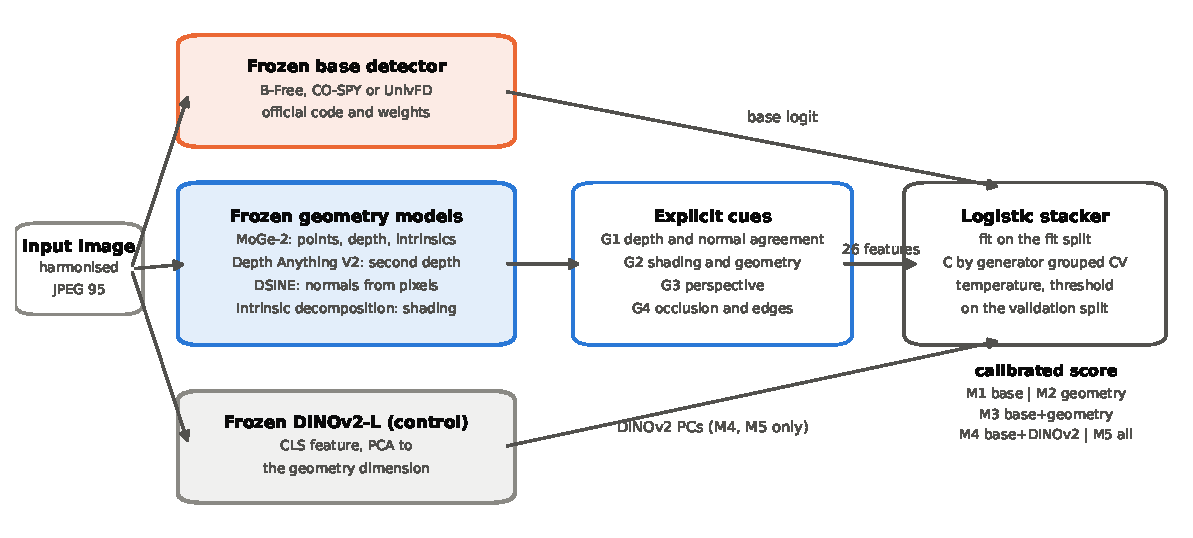
\includegraphics[width=\linewidth]{fig_architecture.pdf}
\caption{Overview. Each image passes through a frozen base detector, four frozen geometry estimators and, for the control models only, a frozen DINOv2 encoder. The geometry outputs are turned into 26 explicit features. A logistic stacker fitted on a separate pool of generators combines the inputs of each model M1 to M5.}
\label{fig:arch}
\end{figure}

\subsection{Geometry estimation}
\label{sec:estimation}

Each image is resized so that its longer side has 640 pixels before geometry estimation. MoGe \citep{wang2025moge} (checkpoint \texttt{moge-2-vitl-normal}) predicts a metric point map $P$, depth $D$, intrinsics $K$ and a validity mask that excludes sky and undefined regions. Estimating $K$ avoids assuming a fixed field of view. Depth Anything V2 Large \citep{yang2024depthanything2} gives a second, independent relative inverse depth $d$. DSINE \citep{bae2024dsine} predicts surface normals $N_{\mathrm{pred}}$ directly from pixels. An ordinal shading decomposition \citep{careaga2023intrinsic} separates the image into albedo $A$ and grey shading $S$, with $I = A \odot S$. Normals are also derived from the point map by the cross product of its central differences,
\begin{equation}
N_D(u,v) = \frac{\partial_u P \times \partial_v P}{\lVert \partial_u P \times \partial_v P \rVert}, \qquad P(u,v) = D(u,v)\,K^{-1}[u,\,v,\,1]^\top .
\label{eq:normals}
\end{equation}
All normals are oriented towards the camera. Because estimators may use different axis conventions, a single sign vector is estimated once on 50 fit images by choosing, among the eight sign flips, the one that minimises the mean angle between $N_{\mathrm{pred}}$ and $N_D$, and it is then held fixed. Pixels within 3 pixels of a depth discontinuity, where $\lVert\nabla \log D\rVert > 0.05$, are excluded, giving the valid set $\Omega$.

\subsection{Four cue groups}
\label{sec:cues}

\paragraph{G1: agreement of depth and normals.} Two independent estimators should agree about surface orientation in a physically real scene; where a scene is geometrically ambiguous, they tend to diverge. For each valid pixel,
\begin{equation}
\theta(p) = \arccos \big\langle N_D(p),\, N_{\mathrm{pred}}(p) \big\rangle ,
\label{eq:theta}
\end{equation}
summarised by its mean, standard deviation and 90th percentile. A second angle uses normals derived from the Depth Anything depth after aligning its inverse depth to MoGe by least squares, $1/D \approx a\,d + c$. We also record the Spearman correlation between $1/D$ and $d$ and the relative error of the affine fit.

\paragraph{G2: consistency of shading and shape.} Under a Lambertian model with distant illumination, shading is well approximated by nine spherical harmonics of the surface normal \citep{ramamoorthi2001efficient},
\begin{equation}
S(p) \approx \sum_{k=1}^{9} \ell_k\, Y_k\big(N_D(p)\big).
\label{eq:sh}
\end{equation}
We fit the lighting vector $\boldsymbol\ell$ with a Huber loss \citep{huber1964robust} by iteratively reweighted least squares, using only pixels in $\Omega$ whose local albedo variation is below the median, which limits the influence of texture and materials:
\begin{equation}
\hat{\boldsymbol\ell} = \arg\min_{\boldsymbol\ell} \sum_{p \in \Omega_A} \rho_{\delta}\Big(S(p) - \mathbf{Y}\big(N_D(p)\big)^{\top}\boldsymbol\ell\Big), \qquad r(p) = S(p) - \mathbf{Y}\big(N_D(p)\big)^{\top}\hat{\boldsymbol\ell}.
\label{eq:huber}
\end{equation}
The threshold $\delta$ is 1.345 times a robust scale of the residuals. Shading is normalised by its median so that residuals are comparable across images. Features are the median and 90th percentile of $|r|$, the coefficient of determination of the fit, and the dispersion of first order lighting vectors fitted separately on a $3\times 3$ grid of regions,
\begin{equation}
\delta_L = \frac{1}{J}\sum_{j=1}^{J} \frac{\lVert \boldsymbol\ell_j - \bar{\boldsymbol\ell}\rVert^2}{\lVert \bar{\boldsymbol\ell}\rVert^2}, \qquad \bar{\boldsymbol\ell} = \frac{1}{J}\sum_{j} \boldsymbol\ell_j ,
\label{eq:dispersion}
\end{equation}
computed when at least four regions have 500 valid pixels. Real scenes can also produce large residuals through mixed lighting, interreflections and specular materials, so G2 is never used as a rule; it is an input whose distribution on real photographs the stacker learns.

\paragraph{G3: perspective consistency.} Line segments are detected with LSD \citep{vongioi2012lsd} at a long side of 1024 pixels and filtered to a length of at least 2.5\% of the diagonal. Up to three vanishing points are fitted by sequential RANSAC, where a segment supports a vanishing point if its direction is within $2^\circ$ of the direction from its midpoint to that point. Features are the number of segments, the number of vanishing points and the length weighted fraction of segments explained by them. When two well supported finite vanishing points correspond to nearly orthogonal directions under the estimated intrinsics (within $10^\circ$), they imply a focal length \citep{hartley2004multiple},
\begin{equation}
f_{VP}^2 = -(\mathbf{v}_1 - \mathbf{c}) \cdot (\mathbf{v}_2 - \mathbf{c}), \qquad \Delta_f = \big|\log f_{VP} - \log f_{\mathrm{MoGe}}\big| ,
\label{eq:focal}
\end{equation}
where $\mathbf{c}$ is the principal point. Vanishing points farther than three image diagonals from $\mathbf{c}$ are rejected because they carry almost no focal information. No Manhattan world assumption is imposed on scenes without such a pair; $\Delta_f$ is then missing.

\paragraph{G4: alignment of occlusions and edges.} An object boundary is both a jump in depth and an edge in the image. With $E_D$ the Canny edges of the log depth and $E_I$ the dilated image edges,
\begin{equation}
A_{\mathrm{occ}} = \frac{|E_D \cap E_I|}{|E_D|},
\label{eq:aocc}
\end{equation}
computed at two edge thresholds (the 85th and 95th percentiles of the gradient magnitude).

\paragraph{Applicability and missing values.} Some cues cannot be computed on every image: a close portrait has few straight lines, and a flat illustration has little depth range. Each group therefore carries indicators (fraction of valid pixels, depth range) and missing value flags. Missing values are imputed with the fit split median. Because a missing flag could itself reveal the class, we report flag rates per class and repeat the analysis without flags (Section~\ref{sec:ablation}). Table~\ref{tab:features} in the appendix lists all 26 features.

\paragraph{Validation on scenes with known geometry.} To verify the implementation, we rendered simple scenes with exact depth, normals and shading, in two versions: a consistent version lit by one light, and an inconsistent version in which each object has its own light and shading follows normals that do not match the 3D shape. Figure~\ref{fig:cues} shows the cue maps and Figure~\ref{fig:synth} the feature distributions over 30 scenes of each kind. The features respond in the expected direction. These renders are not a model of photographs or of generated images; they only show that the code measures what the equations describe.

\begin{figure}[t]
\centering
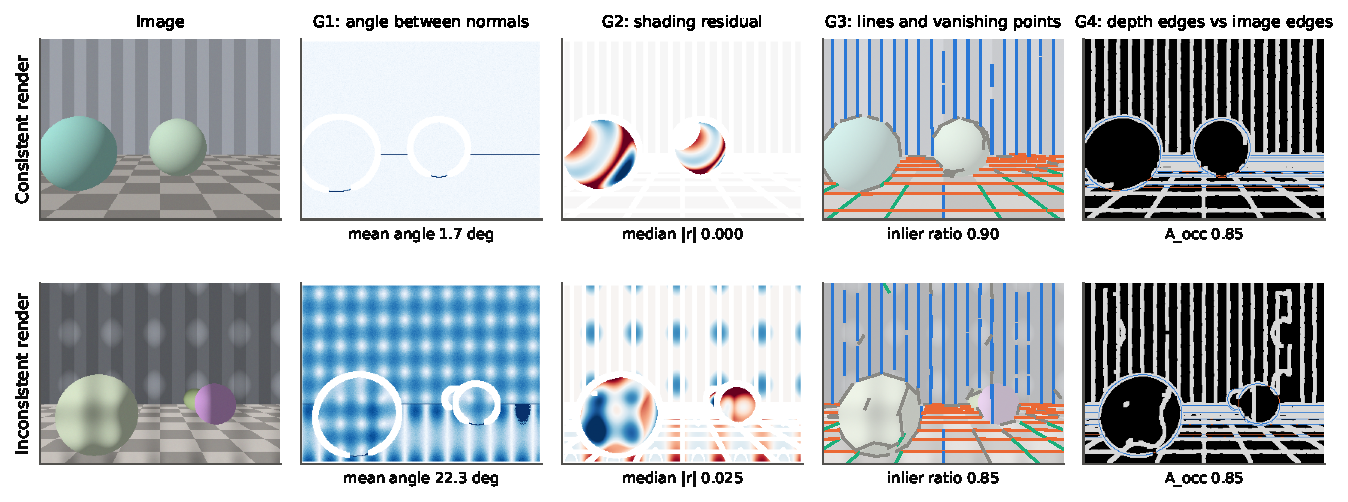
\includegraphics[width=\linewidth]{fig_cues_synthetic.pdf}
\caption{The four cue groups on a consistent and an inconsistent synthetic render with known geometry. G1: angle between normals derived from depth and normals predicted from pixels. G2: residual of the spherical harmonic shading fit (red and blue, positive and negative). G3: line segments coloured by vanishing point. G4: depth edges that coincide with image edges (blue) or do not (orange). These renders only validate the implementation.}
\label{fig:cues}
\end{figure}

\begin{figure}[t]
\centering
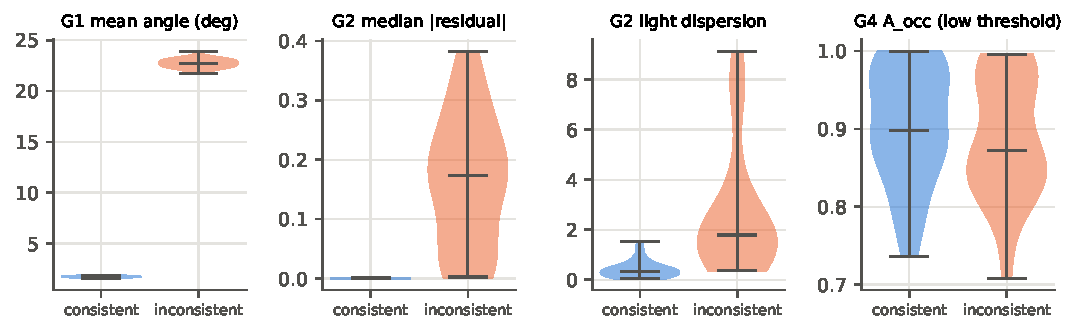
\includegraphics[width=\linewidth]{fig_synthetic_check.pdf}
\caption{Feature distributions on 30 consistent and 30 inconsistent synthetic renders. Implementation check only; it says nothing about real or generated photographs.}
\label{fig:synth}
\end{figure}

\subsection{Calibrated stacker}
\label{sec:stacker}

All five models use the same procedure. Features are imputed and standardised with fit split statistics. The inverse regularisation strength $C \in \{10^{-3},10^{-2},10^{-1},1,10\}$ of an L2 regularised logistic regression is chosen by five fold cross validation on the fit split, where fake images are grouped by generator so that each fold holds out whole generators; the selection therefore rewards transfer to new generators. Among values within 0.001 AUROC of the best, the strongest regularisation is chosen. The model is refitted on the full fit split. Temperature scaling \citep{guo2017calibration} and an operating threshold that yields a 5\% false positive rate on validation real images are then fixed on the validation split. Nothing is fitted on a test set. A gradient boosted tree model with depth at most three serves as a check that conclusions do not depend on the linear form.

\subsection{DINOv2 control}
\label{sec:control}

Depth Anything V2 and MoGe use DINOv2 encoders, and B-Free uses a DINOv2 pretrained backbone. A gain from geometry could therefore be a gain from adding a strong general representation. The control model M4 adds the DINOv2 Large class token \citep{oquab2024dinov2}, reduced by principal component analysis fitted on the fit split to 26 dimensions. The main claim uses only the explicit geometric outputs; we do not feed the geometry models' internal tokens to the stacker, because those tokens are DINOv2 features.

% =====================================================================
\section{Experimental setup}
\label{sec:setup}

\subsection{Data and splits}
\label{sec:data}

All data are existing public datasets; no new images were collected. Figure~\ref{fig:design} and Table~\ref{tab:data} summarise the design. The fit and validation pool contains Co-Spy-Bench images \citep{cheng2025cospy} generated from CC3M captions by ten open models, and real Flickr30k photographs. Four test sets follow.

\begin{figure}[t]
\centering
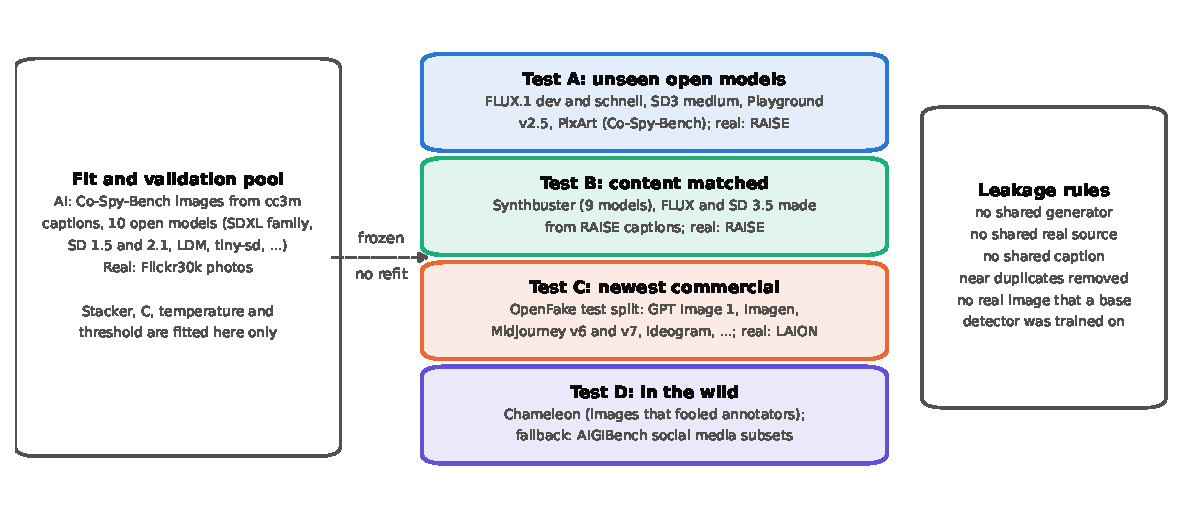
\includegraphics[width=\linewidth]{fig_study_design.pdf}
\caption{Study design. The stacker, its regularisation, temperature and threshold are fitted on the pool at the left only. The four test sets share no generator, real image source or caption with that pool, and no real image comes from a base detector's own training data.}
\label{fig:design}
\end{figure}

\begin{table}[t]
\centering
\caption{Datasets and roles. Counts after capping and deduplication are filled from \texttt{split\_summary.csv}.}
\label{tab:data}
\small
\begin{tabularx}{\linewidth}{@{}l X l l@{}}
\toprule
Set & Generated images (generators) & Real images & Images (real / fake) \\
\midrule
Fit and validation & Co-Spy-Bench, CC3M captions: SSD-1B, tiny-sd, small-sd, SegMoE, LCM LoRA (SDXL and SD 1.5), SDXL Turbo, LDM, SD 1.5, SD 2.1 & Flickr30k & \xyz[data.fitval.n_real]{} / \xyz[data.fitval.n_fake] \\
A: unseen open models & Co-Spy-Bench, TextCaps and SBU captions: FLUX.1-dev, FLUX.1-schnell, SD3 Medium, Playground v2.5, PixArt XL (1024 and 512) & RAISE & \xyz[data.A.n_real]{} / \xyz[data.A.n_fake] \\
B: content matched & Synthbuster \citep{bammey2023synthbuster}: DALL\textperiodcentered E 2 and 3, Firefly, Midjourney v5, GLIDE, SD 1.3, 1.4, 2, XL; extended set: FLUX and SD 3.5 from the same RAISE captions & RAISE & \xyz[data.B.n_real]{} / \xyz[data.B.n_fake] \\
C: newest commercial & OpenFake test split \citep{livernoche2025openfake}: GPT Image 1, Imagen 3 and 4, Midjourney v6 and v7, FLUX 1.1 Pro, Ideogram 3, Grok 2, HiDream, Recraft v3 and others & LAION, Pexels & \xyz[data.C.n_real]{} / \xyz[data.C.n_fake] \\
D: in the wild & Chameleon \citep{yan2025aide} (or AIGIBench social subsets \citep{li2025aigibench}) & Chameleon & \xyz[data.D.n_real]{} / \xyz[data.D.n_fake] \\
\bottomrule
\end{tabularx}
\end{table}

Test A contains open models that none of the base detectors or the fit pool used, compared with RAISE photographs. Test B is the content matched control: Synthbuster images were generated from captions of the RAISE photographs \citep{bammey2023synthbuster}, and an extended release adds FLUX and SD 3.5 images made from the same captions, so real and generated images depict similar scenes. Test C contains the newest commercial systems in the OpenFake test split, which is never used for fitting. Test D contains images collected because they fooled human annotators. Generators of a family seen by any base detector or by the fit pool (Stable Diffusion 1.x and 2.x, the SDXL family, ProGAN and Stable Diffusion fine tunes) are tagged as seen family; the headline analyses use unseen generators only, and seen family results are reported separately.

\paragraph{Leakage controls.} The pipeline refuses to run if any fake generator, real image source or caption appears in both the fit pool and a test set. Near duplicates are removed by a 64 bit perceptual hash with a Hamming threshold of 8; any fit image within that distance of a test image is dropped, and test sets are never altered. Fit and validation images are split by caption so that one caption never appears on both sides. Base detectors bring their own training data (Table~\ref{tab:bases}): B-Free and CO-SPY were trained with MS COCO photographs and UnivFD with LSUN photographs, so no test set contains real images from MS COCO, LSUN or ImageNet.

\begin{table}[t]
\centering
\caption{Base detectors, all frozen and used through their official code and weights.}
\label{tab:bases}
\small
\begin{tabularx}{\linewidth}{@{}l X X@{}}
\toprule
Detector & Family & Training data of the released weights \\
\midrule
B-Free \citep{guillaro2025bfree} & Bias free training; DINOv2 pretrained ViT with registers & 51{,}517 MS COCO photographs and 309{,}102 SD 2.1 inpainted or self conditioned images \\
CO-SPY \citep{cheng2025cospy} & Semantic (CLIP) plus VAE artifact features & DRCT-2M: MS COCO photographs and SD 1.4 images (checkpoint \texttt{sd-v1\_4}) \\
UnivFD \citep{ojha2023univfd} & Frozen CLIP ViT-L/14 with a linear layer & ProGAN images and LSUN photographs \\
\bottomrule
\end{tabularx}
\end{table}

\subsection{Processing and robustness variants}
\label{sec:processing}

Every image, real or generated, is decoded and reencoded as JPEG at quality 95 before any model sees it. This removes the format shortcut described by \citet{grommelt2024fake}. For the robustness analysis, three further copies of every test image are produced from the harmonised image: JPEG at quality 75, bicubic downscaling to half size, and a screenshot chain (downscaling to 0.75 followed by JPEG at quality 80). The base score, the geometry features and the control features are recomputed from each processed copy.

\subsection{Metrics}
\label{sec:metrics}

The primary metric is macro AUROC over unseen generators (Equation~\ref{eq:macro}). The true positive rate at a 1\% false positive rate is a coprimary metric because forensic use tolerates very few false alarms. At the fixed validation threshold we report the false positive rate on real photographs, the accuracy on real and on generated images and their mean, and the expected calibration error with 15 bins,
\begin{equation}
\mathrm{ECE} = \sum_{m=1}^{15} \frac{|B_m|}{n}\, \big|\mathrm{acc}(B_m) - \mathrm{conf}(B_m)\big| .
\label{eq:ece}
\end{equation}

\subsection{Statistical analysis}
\label{sec:stats}

The primary test is a paired, generator level cluster bootstrap \citep{field2007bootstrapping}. Each of 2{,}000 replicates resamples the unseen fake generators and the real image sources with replacement, then resamples images within each, and computes both models' macro AUROC on the same replicate. The 2.5th and 97.5th percentiles of the differences give the 95\% interval. Hypotheses tested across the three base detectors are corrected with the Holm procedure \citep{holm1979simple}. As supplementary image level analyses, we use the DeLong test for AUROC differences \citep{delong1988comparing,sun2014fast} and the McNemar test for accuracy differences at the fixed threshold \citep{mcnemar1947note}; each test is used only for the metric it addresses. A significant gain below 0.01 AUROC is reported as detectable but small. With fewer than five unseen generators in a test set, the bootstrap interval is labelled indicative and per generator results are the main evidence.

\subsection{Implementation and compute}
\label{sec:impl}

The code is written in Python with PyTorch, scikit-learn and OpenCV; all stages are resumable and record their configuration, software versions and timing. The feature code, the stacker, the metrics and the statistics are covered by unit tests, and an end to end smoke test runs the whole pipeline on synthetic renders on a CPU. Geometry extraction and detection ran on \xyz[compute.gpu]{} GPUs. Measured cost per image is reported in Figure~\ref{fig:cost}. Random seeds are fixed; the logistic stacker is deterministic given its data.

\subsection{Pilot study}
\label{sec:pilot}

Before the full study, a pilot with UnivFD as the base detector, cues G1 and G2, Tests A and B (subsampled) and the clean and JPEG 75 copies decided whether to continue. The rule was fixed in advance: proceed if the M3 gain over M1 was at least 0.01 macro AUROC with the lower bound of its 90\% cluster bootstrap interval above zero, if the M3 gain exceeded the M4 gain, and if the extra rise in real photo false positives under JPEG 75 was at most 2 points. If geometry alone (M2) reached 0.65 macro AUROC but the first rule failed, the cues would be revised; otherwise the study would stop and report a negative result.

% =====================================================================
\section{Results}
\label{sec:results}

\subsection{Pilot}

The pilot gave a gain of \xyz[pilot.delta]{} macro AUROC (90\% CI \xyz[pilot.ci90]), an M4 gain of \xyz[pilot.gain_m4]{}, an extra false positive drift of \xyz[pilot.extra_fpr_drift]{} points and an M2 macro AUROC of \xyz[pilot.m2_auroc]{}. The preregistered decision was \xyz[pilot.decision].

\subsection{Does geometry add to existing detectors? (H1)}

Table~\ref{tab:main} and Figure~\ref{fig:models} compare the five models on the four test sets. Pooled over all unseen generators, adding geometry changed macro AUROC by \xyz[h1.bfree.delta]{} for B-Free (95\% CI \xyz[h1.bfree.ci], Holm adjusted $p$ \xyz[h1.bfree.p]), \xyz[h1.cospy.delta]{} for CO-SPY (\xyz[h1.cospy.ci], \xyz[h1.cospy.p]) and \xyz[h1.univfd.delta]{} for UnivFD (\xyz[h1.univfd.ci], \xyz[h1.univfd.p]). Hypothesis H1 was therefore \xyz[h1.verdict]. Geometry alone (M2) reached \xyz[m2.macro_auroc]{} macro AUROC. Figure~\ref{fig:roc} shows that the change at low false positive rates was \xyz[h1.tpr_summary].

\begin{table}[t]
\centering
\caption{Macro AUROC / TPR at 1\% FPR on unseen generators (clean copies). Best value per detector and test set in bold.}
\label{tab:main}
\small
\begin{tabular}{@{}llcccc@{}}
\toprule
Detector & Model & A: open models & B: content matched & C: commercial & D: in the wild \\
\midrule
\multirow{5}{*}{B-Free} & M1 base & \xyz[main.bfree.M1.A] & \xyz[main.bfree.M1.B] & \xyz[main.bfree.M1.C] & \xyz[main.bfree.M1.D] \\
 & M2 geometry & \xyz[main.bfree.M2.A] & \xyz[main.bfree.M2.B] & \xyz[main.bfree.M2.C] & \xyz[main.bfree.M2.D] \\
 & M3 base + geometry & \xyz[main.bfree.M3.A] & \xyz[main.bfree.M3.B] & \xyz[main.bfree.M3.C] & \xyz[main.bfree.M3.D] \\
 & M4 base + DINOv2 & \xyz[main.bfree.M4.A] & \xyz[main.bfree.M4.B] & \xyz[main.bfree.M4.C] & \xyz[main.bfree.M4.D] \\
 & M5 all & \xyz[main.bfree.M5.A] & \xyz[main.bfree.M5.B] & \xyz[main.bfree.M5.C] & \xyz[main.bfree.M5.D] \\
\midrule
\multirow{5}{*}{CO-SPY} & M1 base & \xyz[main.cospy.M1.A] & \xyz[main.cospy.M1.B] & \xyz[main.cospy.M1.C] & \xyz[main.cospy.M1.D] \\
 & M2 geometry & \xyz[main.cospy.M2.A] & \xyz[main.cospy.M2.B] & \xyz[main.cospy.M2.C] & \xyz[main.cospy.M2.D] \\
 & M3 base + geometry & \xyz[main.cospy.M3.A] & \xyz[main.cospy.M3.B] & \xyz[main.cospy.M3.C] & \xyz[main.cospy.M3.D] \\
 & M4 base + DINOv2 & \xyz[main.cospy.M4.A] & \xyz[main.cospy.M4.B] & \xyz[main.cospy.M4.C] & \xyz[main.cospy.M4.D] \\
 & M5 all & \xyz[main.cospy.M5.A] & \xyz[main.cospy.M5.B] & \xyz[main.cospy.M5.C] & \xyz[main.cospy.M5.D] \\
\midrule
\multirow{5}{*}{UnivFD} & M1 base & \xyz[main.univfd.M1.A] & \xyz[main.univfd.M1.B] & \xyz[main.univfd.M1.C] & \xyz[main.univfd.M1.D] \\
 & M2 geometry & \xyz[main.univfd.M2.A] & \xyz[main.univfd.M2.B] & \xyz[main.univfd.M2.C] & \xyz[main.univfd.M2.D] \\
 & M3 base + geometry & \xyz[main.univfd.M3.A] & \xyz[main.univfd.M3.B] & \xyz[main.univfd.M3.C] & \xyz[main.univfd.M3.D] \\
 & M4 base + DINOv2 & \xyz[main.univfd.M4.A] & \xyz[main.univfd.M4.B] & \xyz[main.univfd.M4.C] & \xyz[main.univfd.M4.D] \\
 & M5 all & \xyz[main.univfd.M5.A] & \xyz[main.univfd.M5.B] & \xyz[main.univfd.M5.C] & \xyz[main.univfd.M5.D] \\
\bottomrule
\end{tabular}
\end{table}

\begin{figure}[t]
\centering
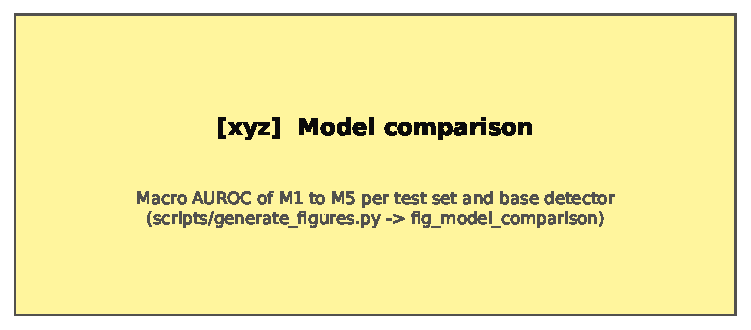
\includegraphics[width=\linewidth]{fig_model_comparison.pdf}
\caption{Macro AUROC over unseen generators for models M1 to M5, per test set and base detector.}
\label{fig:models}
\end{figure}

\begin{figure}[t]
\centering
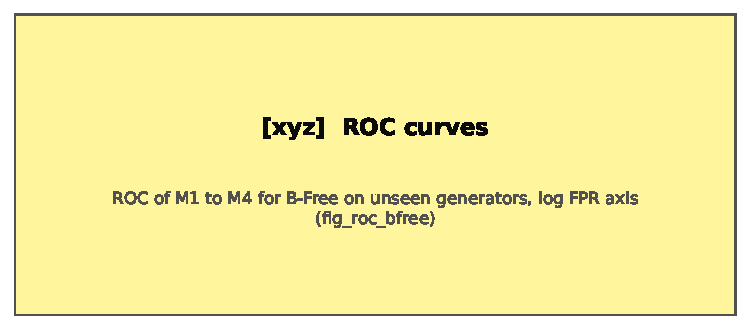
\includegraphics[width=0.55\linewidth]{fig_roc_bfree.pdf}
\caption{ROC curves of M1 to M4 with B-Free as the base detector, unseen generators, logarithmic false positive axis. Curves for CO-SPY and UnivFD are in the supplementary material.}
\label{fig:roc}
\end{figure}

\subsection{Which generators benefit?}

Figure~\ref{fig:pergen} shows the gain for each test generator. The gain was largest for \xyz[pergen.largest]{} and smallest for \xyz[pergen.smallest]. Seen family generators, reported separately, showed a gain of \xyz[pergen.seen_family_gain].

\begin{figure}[t]
\centering
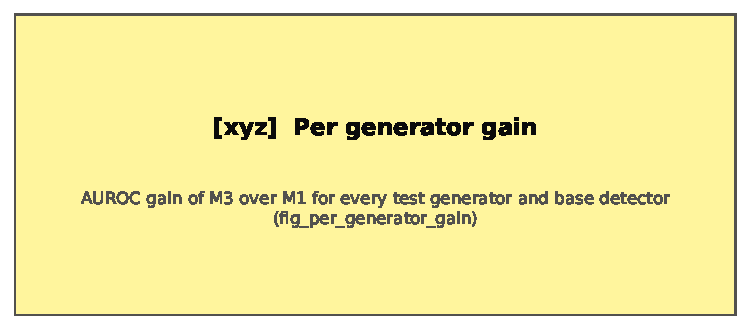
\includegraphics[width=\linewidth]{fig_per_generator_gain.pdf}
\caption{AUROC gain of M3 over M1 for every test generator (each generator's images against all real images of its test set). One marker per base detector.}
\label{fig:pergen}
\end{figure}

\subsection{Is the gain geometric? (H2, H3)}

Against the DINOv2 control, M3 differed from M4 by \xyz[h2.bfree.delta]{} macro AUROC for B-Free (95\% CI \xyz[h2.bfree.ci]), \xyz[h2.cospy.delta]{} for CO-SPY and \xyz[h2.univfd.delta]{} for UnivFD, so H2 was \xyz[h2.verdict]. On the content matched Test B the gain was \xyz[h3.bfree.delta]{} (\xyz[h3.bfree.ci]), \xyz[h3.cospy.delta]{} and \xyz[h3.univfd.delta], so H3 was \xyz[h3.verdict]. Table~\ref{tab:hyptests} lists all tests.

\begin{table}[t]
\centering
\caption{Hypothesis tests on unseen generators: estimate, 95\% generator level cluster bootstrap interval and Holm adjusted $p$ value.}
\label{tab:hyptests}
\small
\begin{tabular}{@{}llccc@{}}
\toprule
Test & Detector & Estimate & 95\% CI & $p$ \\
\midrule
H1 (M3 vs M1) & B-Free & \xyz[h1.bfree.delta] & \xyz[h1.bfree.ci] & \xyz[h1.bfree.p] \\
 & CO-SPY & \xyz[h1.cospy.delta] & \xyz[h1.cospy.ci] & \xyz[h1.cospy.p] \\
 & UnivFD & \xyz[h1.univfd.delta] & \xyz[h1.univfd.ci] & \xyz[h1.univfd.p] \\
H2 (M3 vs M4) & B-Free & \xyz[h2.bfree.delta] & \xyz[h2.bfree.ci] & \xyz[h2.bfree.p] \\
 & CO-SPY & \xyz[h2.cospy.delta] & \xyz[h2.cospy.ci] & \xyz[h2.cospy.p] \\
 & UnivFD & \xyz[h2.univfd.delta] & \xyz[h2.univfd.ci] & \xyz[h2.univfd.p] \\
H3 (Test B) & B-Free & \xyz[h3.bfree.delta] & \xyz[h3.bfree.ci] & \xyz[h3.bfree.p] \\
 & CO-SPY & \xyz[h3.cospy.delta] & \xyz[h3.cospy.ci] & \xyz[h3.cospy.p] \\
 & UnivFD & \xyz[h3.univfd.delta] & \xyz[h3.univfd.ci] & \xyz[h3.univfd.p] \\
\bottomrule
\end{tabular}
\end{table}

\subsection{Robustness to processing (H4)}

Figure~\ref{fig:robust} and Table~\ref{tab:robust} show the effect of processing. Under JPEG 75 the gain was \xyz[h4.jpeg75.range], under half resizing \xyz[h4.resize05.range]{} and under the screenshot chain \xyz[h4.screenshot.range]. Under JPEG 75, the real photo false positive rate at the fixed threshold rose on average over the three detectors by \xyz[h4.jpeg75.fpr_drift_m1]{} points for M1 and \xyz[h4.jpeg75.fpr_drift_m3]{} points for M3. Figure~\ref{fig:shift} shows which geometry features moved most under processing: \xyz[shift.top_feature]{} shifted by \xyz[shift.top_smd]{} standard deviations on real photographs under JPEG 75.

\begin{table}[t]
\centering
\caption{Gain of M3 over M1 (macro AUROC, 95\% CI) and extra false positive drift on real photographs under processing.}
\label{tab:robust}
\small
\begin{tabular}{@{}lccc@{}}
\toprule
Detector & JPEG 75 & Half resize & Screenshot chain \\
\midrule
B-Free & \xyz[h4.bfree.jpeg75.delta]{} (\xyz[h4.bfree.jpeg75.ci]) & \xyz[h4.bfree.resize05.delta]{} (\xyz[h4.bfree.resize05.ci]) & \xyz[h4.bfree.screenshot.delta]{} (\xyz[h4.bfree.screenshot.ci]) \\
CO-SPY & \xyz[h4.cospy.jpeg75.delta]{} (\xyz[h4.cospy.jpeg75.ci]) & \xyz[h4.cospy.resize05.delta]{} (\xyz[h4.cospy.resize05.ci]) & \xyz[h4.cospy.screenshot.delta]{} (\xyz[h4.cospy.screenshot.ci]) \\
UnivFD & \xyz[h4.univfd.jpeg75.delta]{} (\xyz[h4.univfd.jpeg75.ci]) & \xyz[h4.univfd.resize05.delta]{} (\xyz[h4.univfd.resize05.ci]) & \xyz[h4.univfd.screenshot.delta]{} (\xyz[h4.univfd.screenshot.ci]) \\
Extra FPR drift (points) & \xyz[h4.jpeg75.extra_fpr_drift] & \xyz[h4.resize05.extra_fpr_drift] & \xyz[h4.screenshot.extra_fpr_drift] \\
\bottomrule
\end{tabular}
\end{table}

\begin{figure}[t]
\centering
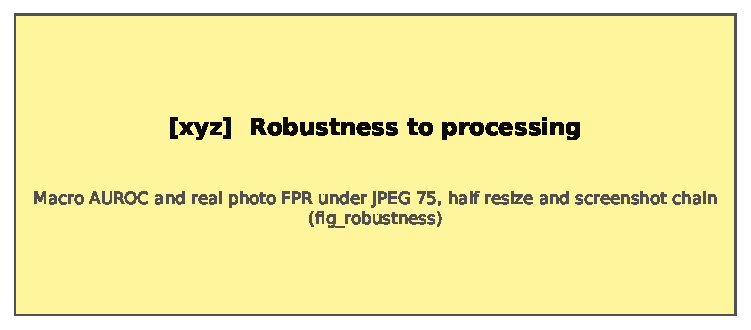
\includegraphics[width=\linewidth]{fig_robustness.pdf}
\caption{Left: macro AUROC on unseen generators for M1 (dashed) and M3 (solid) across processing. Right: share of real photographs flagged at the threshold fixed on validation data.}
\label{fig:robust}
\end{figure}

\begin{figure}[t]
\centering
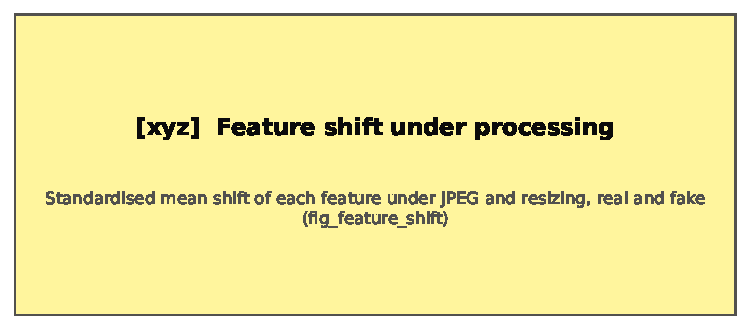
\includegraphics[width=\linewidth]{fig_feature_shift.pdf}
\caption{Standardised mean shift of each geometry feature between clean and processed copies, for real and generated test images separately.}
\label{fig:shift}
\end{figure}

\subsection{Ablation study}
\label{sec:ablation}

Each ablation changes one component of M3 and keeps everything else fixed: the same splits, base scores, stacker procedure, seeds and test images. Table~\ref{tab:ablation} and Figure~\ref{fig:ablation} report the change in pooled macro AUROC against the full M3 with 95\% cluster bootstrap intervals. Removing a cue group tests whether it contributes beyond the others; keeping a single group tests whether it carries signal alone; removing the missing value flags tests whether missingness leaks class information; the tree model tests the linear form; fitting on processed copies tests whether robustness can be gained without touching test data; and replacing DSINE normals with Marigold normals \citep{ke2024marigold} or the ordinal shading with a Retinex estimate tests sensitivity to the estimators.

\begin{table}[t]
\centering
\caption{Ablations of M3: change in pooled macro AUROC on unseen generators (95\% CI).}
\label{tab:ablation}
\small
\begin{tabular}{@{}lccc@{}}
\toprule
Ablation & B-Free & CO-SPY & UnivFD \\
\midrule
Without G1 (depth and normals) & \xyz[abl.drop_G1.bfree] & \xyz[abl.drop_G1.cospy] & \xyz[abl.drop_G1.univfd] \\
Without G2 (shading) & \xyz[abl.drop_G2.bfree] & \xyz[abl.drop_G2.cospy] & \xyz[abl.drop_G2.univfd] \\
Without G3 (perspective) & \xyz[abl.drop_G3.bfree] & \xyz[abl.drop_G3.cospy] & \xyz[abl.drop_G3.univfd] \\
Without G4 (occlusion edges) & \xyz[abl.drop_G4.bfree] & \xyz[abl.drop_G4.cospy] & \xyz[abl.drop_G4.univfd] \\
Only G1 & \xyz[abl.only_G1.bfree] & \xyz[abl.only_G1.cospy] & \xyz[abl.only_G1.univfd] \\
Only G2 & \xyz[abl.only_G2.bfree] & \xyz[abl.only_G2.cospy] & \xyz[abl.only_G2.univfd] \\
Only G3 & \xyz[abl.only_G3.bfree] & \xyz[abl.only_G3.cospy] & \xyz[abl.only_G3.univfd] \\
Only G4 & \xyz[abl.only_G4.bfree] & \xyz[abl.only_G4.cospy] & \xyz[abl.only_G4.univfd] \\
Without missing value flags & \xyz[abl.no_flags.bfree] & \xyz[abl.no_flags.cospy] & \xyz[abl.no_flags.univfd] \\
Gradient boosted trees & \xyz[abl.gbdt.bfree] & \xyz[abl.gbdt.cospy] & \xyz[abl.gbdt.univfd] \\
Fitted with processed copies & \xyz[abl.processing_aware_fit.bfree] & \xyz[abl.processing_aware_fit.cospy] & \xyz[abl.processing_aware_fit.univfd] \\
Marigold normals instead of DSINE & \xyz[abl.estimator_features_marigold.bfree] & \xyz[abl.estimator_features_marigold.cospy] & \xyz[abl.estimator_features_marigold.univfd] \\
Retinex shading instead of ordinal shading & \xyz[abl.estimator_features_retinex.bfree] & \xyz[abl.estimator_features_retinex.cospy] & \xyz[abl.estimator_features_retinex.univfd] \\
\bottomrule
\end{tabular}
\end{table}

\begin{figure}[t]
\centering
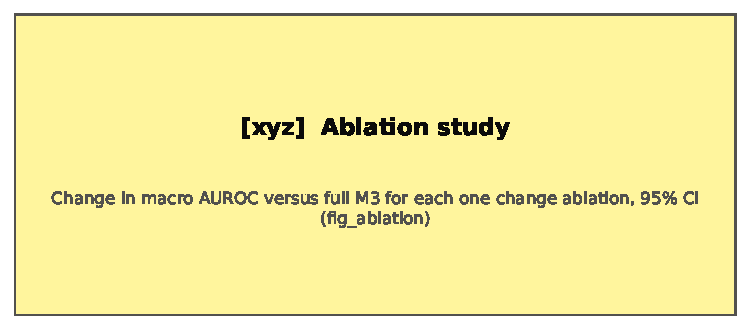
\includegraphics[width=\linewidth]{fig_ablation.pdf}
\caption{Ablations of M3. Markers show the change in pooled macro AUROC against the full model; bars are 95\% cluster bootstrap intervals.}
\label{fig:ablation}
\end{figure}

\subsection{Scene types (H5) and feature behaviour}

Figure~\ref{fig:scene} breaks the gain down by scene label. The largest gain appeared for \xyz[scene.largest]{} scenes and the smallest for \xyz[scene.smallest]. Figure~\ref{fig:dist} shows the distributions of six features on real and generated test images.

\begin{figure}[t]
\centering
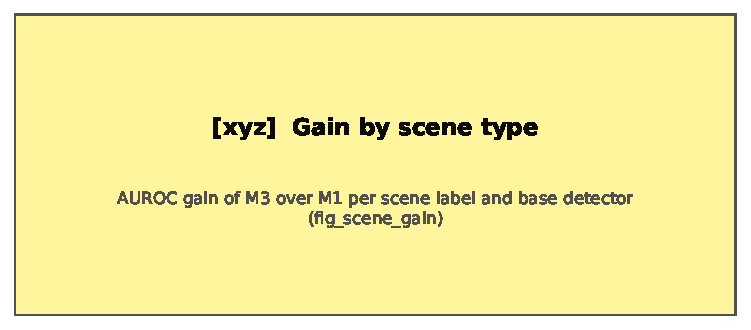
\includegraphics[width=0.7\linewidth]{fig_scene_gain.pdf}
\caption{AUROC gain of M3 over M1 by scene label (zero shot CLIP labels, audited on 300 images, Cohen's $\kappa$ = \xyz[scene.kappa]). Scene classes with fewer than 200 images per label are omitted.}
\label{fig:scene}
\end{figure}

\begin{figure}[t]
\centering
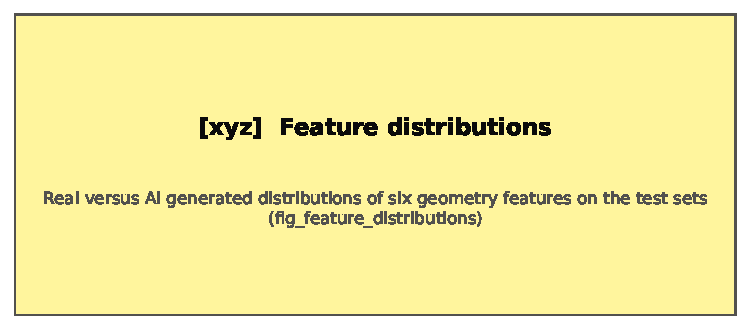
\includegraphics[width=\linewidth]{fig_feature_distributions.pdf}
\caption{Distributions of six geometry features on real (blue) and generated (orange) test images, clean copies.}
\label{fig:dist}
\end{figure}

\subsection{Qualitative examples and error analysis}

Figure~\ref{fig:qual} shows real and generated images from Test B with their geometry maps. \xyz[manual.qualitative]{} [Describe what the maps show for correctly detected images, then for the false positives and false negatives of M3, using the saved maps of the misclassified images.] The most common false positives were \xyz[manual.common_fp]{} and the most common false negatives were \xyz[manual.common_fn].

\begin{figure}[t]
\centering
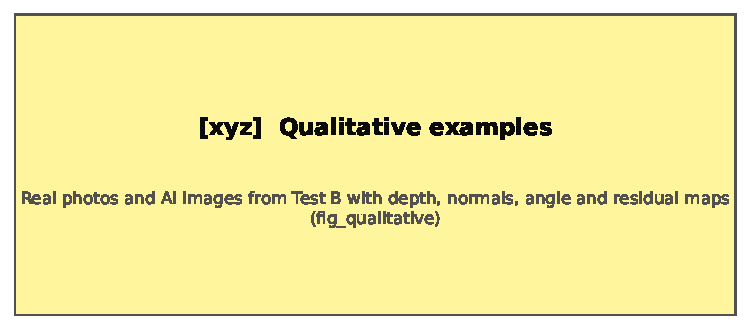
\includegraphics[width=\linewidth]{fig_qualitative.pdf}
\caption{Correctly classified real photographs and generated images from Test B, followed by the most confident false positive and false negative of M3, with depth, normals derived from depth, predicted normals, the angle between them, and the shading residual.}
\label{fig:qual}
\end{figure}

\subsection{Compute cost}

\begin{figure}[t]
\centering
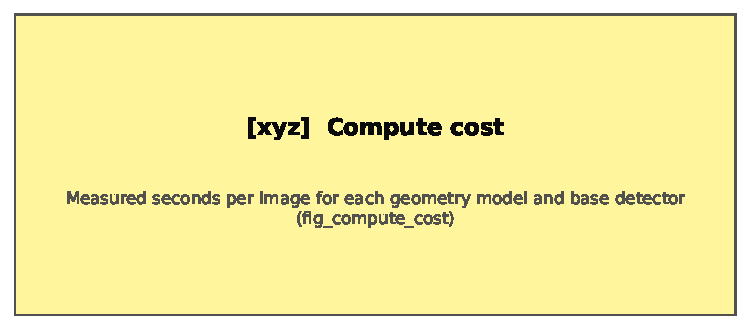
\includegraphics[width=0.75\linewidth]{fig_compute_cost.pdf}
\caption{Measured seconds per image for the geometry models, the feature computation and each base detector on \xyz[compute.gpu].}
\label{fig:cost}
\end{figure}

Geometry extraction took \xyz[compute.geom_sec]{} seconds per image on \xyz[compute.gpu], of which feature computation was \xyz[compute.feat_sec]{} seconds (Figure~\ref{fig:cost}). The base detectors took \xyz[compute.det_min]{} to \xyz[compute.det_max]{} seconds per image.

% =====================================================================
\section{Discussion}
\label{sec:discussion}

[Write this section after the results are in. Keep the conclusions tied to the hypotheses that passed or failed, and use the guide below.]

\paragraph{If H1 to H4 pass.} Explicit geometry carries information that the three base detectors do not capture, the information is not explained by backbone features or content, and it survives common processing. The per cue ablation (Table~\ref{tab:ablation}) indicates which physical constraint generators violate most, and the scene analysis indicates where the cue applies.

\paragraph{If H1 passes but H2 or H3 fails.} The gain exists but cannot be attributed to geometry. Report it as a cautionary result: features from geometry models can encode backbone semantics or content and style, and studies of physical forensics need the controls used here.

\paragraph{If H4 fails.} Geometry estimates degrade under compression and resizing, so the gain is fragile in practice even if it is real on clean images.

\paragraph{If H1 fails.} Current detectors already capture what these explicit cues measure, or modern generators produce geometry that monocular estimators cannot distinguish from real scenes. Either reading is useful to the field.

In all cases, the generator level intervals describe uncertainty about new generators from the same period; they cannot guarantee performance on generators released later.

% =====================================================================
\section{Limitations and threats to validity}
\label{sec:limits}

\paragraph{Estimator bias.} The geometry models were trained partly on rendered data, and their errors may differ between real and generated images for reasons unrelated to physics. We report this as a confound and test sensitivity by swapping estimators, but we cannot remove it.

\paragraph{Construct validity.} A large shading residual or disagreement between normals is not proof of generation; real scenes with mixed lighting or complex materials produce the same signals. The features are used only as learned inputs, never as rules.

\paragraph{Content matching.} Synthbuster images were generated from captions of RAISE photographs, so they depict similar but not identical scenes. True pairs of a real photograph and a generated image of the same scene are not available in public data.

\paragraph{External validity.} The test sets cover \xyz[ext.n_unseen_generators]{} unseen generators from \xyz[ext.earliest]{} to \xyz[ext.latest]. Images from later generators, partially edited images (inpainting, composites, face swaps) and adversarially perturbed images are outside the scope of this study.

\paragraph{Data access.} Chameleon is available on request; OpenFake real images are distributed as links and some were no longer reachable (\xyz[manual.openfake_retrieved]{} of \xyz[manual.openfake_requested]{} retrieved).

\paragraph{Statistical power.} With \xyz[ext.n_unseen_generators]{} unseen generators, cluster bootstrap intervals are wide; per generator results are reported for this reason.

% =====================================================================
\section{Ethical considerations}

The study uses only public datasets under their licences, several of which restrict use to noncommercial research. No new images of people were created. Detector outputs are probabilistic and come with calibrated scores; they should support, not replace, human judgement, and false positive rates on real photographs are reported so that the risk of wrongly accusing someone of fabrication can be assessed. Because detection research can inform evasion, we do not release adversarial methods.

% =====================================================================
\section{Conclusion}
\label{sec:conclusion}

We asked whether explicit monocular 3D geometry helps existing detectors of AI generated images on generators they have never seen. Using 26 physically interpretable features from frozen estimators, three released detectors, four leakage controlled test sets and preregistered tests with generator level inference, we found \xyz[manual.conclusion]. [Summarise in two sentences which hypotheses passed.] Future work includes fusing geometry with reconstruction and semantic cues, evaluating adversarial robustness of such multi cue detectors, localising edits in partially generated images with regional geometry, and grounding the explanations of multimodal models in measured geometric evidence.

% =====================================================================
\section*{Data and code availability}
Code, configuration files, split definitions and per image feature tables are available at [repository URL]. The datasets are available from their original providers under their own licences (Synthbuster, Zenodo record 10066460; extended Synthbuster, GRIP UNINA; Co-Spy-Bench, Hugging Face; Flickr30k, Hugging Face; OpenFake, Hugging Face; Chameleon, on request from its authors).

\section*{Declaration of generative AI use}
[State how AI assistance was used in preparing the code and manuscript, as required by the journal. Example: During the preparation of this work the authors used an AI assistant to draft code and text. The authors reviewed and edited all content and take full responsibility for it.]

\section*{Funding}
[Funding sources, or: This research received no specific grant from any funding agency.]

\section*{Conflict of interest}
[The authors declare no competing interests.]

\section*{Author contributions}
[CRediT statement.]

\bibliographystyle{plainnat}
\bibliography{references}

% =====================================================================
\appendix
\section{Feature list}
\label{app:features}

\begin{table}[h]
\centering
\caption{The 26 explicit geometry features (names as in the released feature tables).}
\label{tab:features}
\small
\begin{tabularx}{\linewidth}{@{}l l X@{}}
\toprule
Group & Feature & Definition \\
\midrule
G1 & \feat{g1\_theta\_mean}, \feat{\_sd}, \feat{\_p90} & Mean, standard deviation and 90th percentile of $\theta$ (Eq.~\ref{eq:theta}), degrees \\
G1 & \feat{g1\_theta\_da\_mean}, \feat{\_p90} & Same angle with normals from aligned Depth Anything depth \\
G1 & \feat{g1\_depth\_rank\_corr} & Spearman correlation of $1/D$ (MoGe) and $d$ (Depth Anything) \\
G1 & \feat{g1\_depth\_affine\_rel\_rmse} & Relative error of the affine fit $1/D \approx a d + c$ \\
G2 & \feat{g2\_res\_median}, \feat{g2\_res\_p90} & Median and 90th percentile of $|r|$ (Eq.~\ref{eq:huber}) \\
G2 & \feat{g2\_sh\_r2} & Coefficient of determination of the shading fit \\
G2 & \feat{g2\_light\_dispersion}, \feat{g2\_n\_regions} & $\delta_L$ (Eq.~\ref{eq:dispersion}) and number of usable regions \\
G3 & \feat{g3\_log\_n\_lines}, \feat{g3\_n\_vp} & Log number of segments, number of vanishing points \\
G3 & \feat{g3\_inlier\_ratio} & Length weighted fraction of segments explained by vanishing points \\
G3 & \feat{g3\_delta\_f} & $\Delta_f$ (Eq.~\ref{eq:focal}) \\
G4 & \feat{g4\_aocc\_lo}, \feat{\_hi}, \feat{\_mean} & $A_{\mathrm{occ}}$ (Eq.~\ref{eq:aocc}) at two thresholds and their mean \\
Indicators & \feat{app\_valid\_frac}, \feat{app\_depth\_range} & Fraction of valid pixels; log ratio of 95th to 5th depth percentile \\
Flags & \feat{miss\_g2}, \feat{miss\_g2\_regions}, \feat{miss\_g3}, \feat{miss\_g3\_f}, \feat{miss\_g4} & 1 when the cue could not be computed \\
\bottomrule
\end{tabularx}
\end{table}

\section{Implementation details}
\label{app:impl}

\begin{table}[h]
\centering
\caption{Models, checkpoints and settings.}
\small
\begin{tabularx}{\linewidth}{@{}l X@{}}
\toprule
Component & Setting \\
\midrule
MoGe & \texttt{Ruicheng/moge-2-vitl-normal}, input long side 640 \\
Depth Anything V2 & \texttt{depth-anything/Depth-Anything-V2-Large-hf} \\
Normals & DSINE via \texttt{hugoycj/DSINE-hub}; ablation: \texttt{prs-eth/marigold-normals-v1-1}, 4 steps \\
Shading & Ordinal shading decomposition (\texttt{compphoto/Intrinsic}, v2); ablation: Retinex \\
DINOv2 control & \texttt{facebook/dinov2-large}, class token, PCA to 26 dimensions on the fit split \\
Scene labels & \texttt{openai/clip-vit-large-patch14}, prompt ensembles, minimum confidence 0.4 \\
Stacker & L2 logistic regression, $C$ grid $\{10^{-3},\dots,10\}$, 5 fold generator grouped CV, temperature scaling, threshold at 5\% validation FPR \\
Statistics & 2{,}000 cluster bootstrap replicates, $\alpha = 0.05$, Holm correction \\
Deduplication & 64 bit DCT perceptual hash, Hamming distance at most 8 \\
\bottomrule
\end{tabularx}
\end{table}

\end{document}
